\section{问题二：流失预测模型与关键因子识别}

在问题一构建的流失客户画像基础上，本节的目标是建立一个能够
量化各特征对流失风险的贡献程度的预测模型，以回答题目提出的
核心问题：哪些因素是驱动客户流失的关键原因？为此，
本文按"数据准备 → 模型建立 → 模型验证与对比 → 关键因子识别"
四个阶段依次推进。

\subsection{数据准备}

在进入建模之前，需将问题一中清洗后的原始数据转换为分类模型
可接受的数值格式。按以下三步依次进行。

\subsubsection*{特征筛选}

基于问题一的 EDA 结论和特征自身的性质，剔除四类无建模价值的列：
与目标变量等价的冗余列（Churn Label）、基于已知流失信息计算的
泄露列（Churn Score，其与 Churn Value 的相关系数高达 0.665）、
仅少数样本有值的单边列（Churn Reason），以及在相关性分析中确认
与流失无线性关联的地理位置列（Latitude、Longitude、Lat Long、
State、City、Zip Code，相关系数均小于 0.01）。
共剔除 9 列，保留 20 个候选特征。

\subsubsection*{类别编码与数值标准化}

16 个分类特征中，二分类变量（Gender、Senior Citizen、Partner、
Dependents、Phone Service、Paperless Billing）取值仅两种，
直接采用 Label 编码映射为 0/1。多分类变量（Contract、Internet
Service、Payment Method、Multiple Lines、Online Security、
Online Backup、Device Protection、Tech Support、Streaming TV、
Streaming Movies）各取值之间不存在天然的序关系——例如合同类型
"月付、一年、两年"只是三类不同期限，并非等距的顺序尺度——
因此不宜使用 Label 编码，而是采用 One-Hot 编码并设置
\texttt{drop\_first=True} 以避免多重共线性。
编码后特征维度由 20 列扩展为 31 列。

4 个数值特征（Tenure Months、Monthly Charges、Total Charges、
CLTV）的量纲和取值范围各不相同。为使各特征在模型训练中
得到平等对待、消除量纲差异的影响，本文采用 Z-score 标准化
将各数值特征的均值和标准差分别调整为 0 和 1。

\subsubsection*{数据集划分}

按 8:2 比例划分训练集与测试集。划分时设置
\texttt{stratify=y}，保证两边的流失率保持一致（均为 26.54\%）。
最终得到训练集 5634 条、测试集 1409 条，编码后的特征维度
为 31 列。

至此，原始数据已转化为包含 31 个标准化特征的数值矩阵，
可输入分类模型进行训练和评估。

\subsection{逻辑回归模型建立}

\subsubsection*{Step 1：模型选择与原理}

逻辑回归（Logistic Regression）是二分类问题中应用最广泛的
统计学习方法之一 \cite{li2019statistical}。它的输出值严格
介于 0 和 1 之间，可解释为样本属于正类的概率，且每个特征的
回归系数 $\beta_j$ 直接反映了该特征对流失概率的影响方向
（系数符号）与强度（绝对值大小），这使得逻辑回归在需要向
非技术背景的业务方解释建模结论时具有天然优势。

本文优先采用逻辑回归作为基线模型，主要基于两点考虑。
第一，问题一的 EDA 已表明流失与各特征之间以线性关系为主：
在网时长与流失的相关系数为 $-0.352$，月消费金额为 $+0.193$，
而更为复杂的非线性交互信号并不突出。第二，问题二的核心要求
不仅在于预测精度，更在于识别关键流失因素并给出合理的业务解释，
逻辑回归的系数可解释性恰好满足这一要求。

逻辑回归假设客户流失概率 $P(Y=1 \mid X)$ 满足 Sigmoid 函数映射：
\begin{equation}
    P(Y=1 \mid X)
    = \frac{1}{1 + e^{-(\beta_0 + \beta_1 x_1 + \cdots + \beta_p x_p)}}
    \label{eq:sigmoid}
\end{equation}
其中 $\beta_0$ 为截距项，$\beta_j$ 为第 $j$ 个特征的回归系数。
模型的参数通过最大化带 $\ell_2$ 正则化的对数似然函数来估计：
\begin{equation}
    \ell = \sum_{i=1}^{N} \left[
        y_i \ln P_i + (1 - y_i) \ln (1 - P_i)
    \right] - \lambda \|\beta\|^2
    \label{eq:loglik}
\end{equation}

\subsubsection*{Step 2：模型训练}

本文使用 scikit-learn 的 LogisticRegression 实现，
通过求解式 \eqref{eq:loglik} 的对数似然函数完成参数估计。

此外，问题一的整体流失率分析（26.54\%）已确认数据存在类别
不平衡问题。为避免模型在训练中过度偏向多数类（未流失客户），
本文设置 \texttt{class\_weight='balanced'}，使模型根据各类别的
样本数量自动调整损失权重，加大对少数类（流失客户）误判的
惩罚力度。

\subsubsection*{Step 3：模型评估}

逻辑回归在测试集上的预测结果如表 \ref{tab:lr_metrics} 所示。

\begin{table}[H]
    \centering
    \caption{逻辑回归模型评估指标}
    \label{tab:lr_metrics}
    \begin{tabular}{ccccc}
        \toprule
        Accuracy & Precision & Recall & F1-score & AUC \\
        \midrule
        0.742    & 0.51      & 0.78   & 0.62     & 0.849 \\
        \bottomrule
    \end{tabular}
\end{table}

\begin{figure}[H]
    \centering
    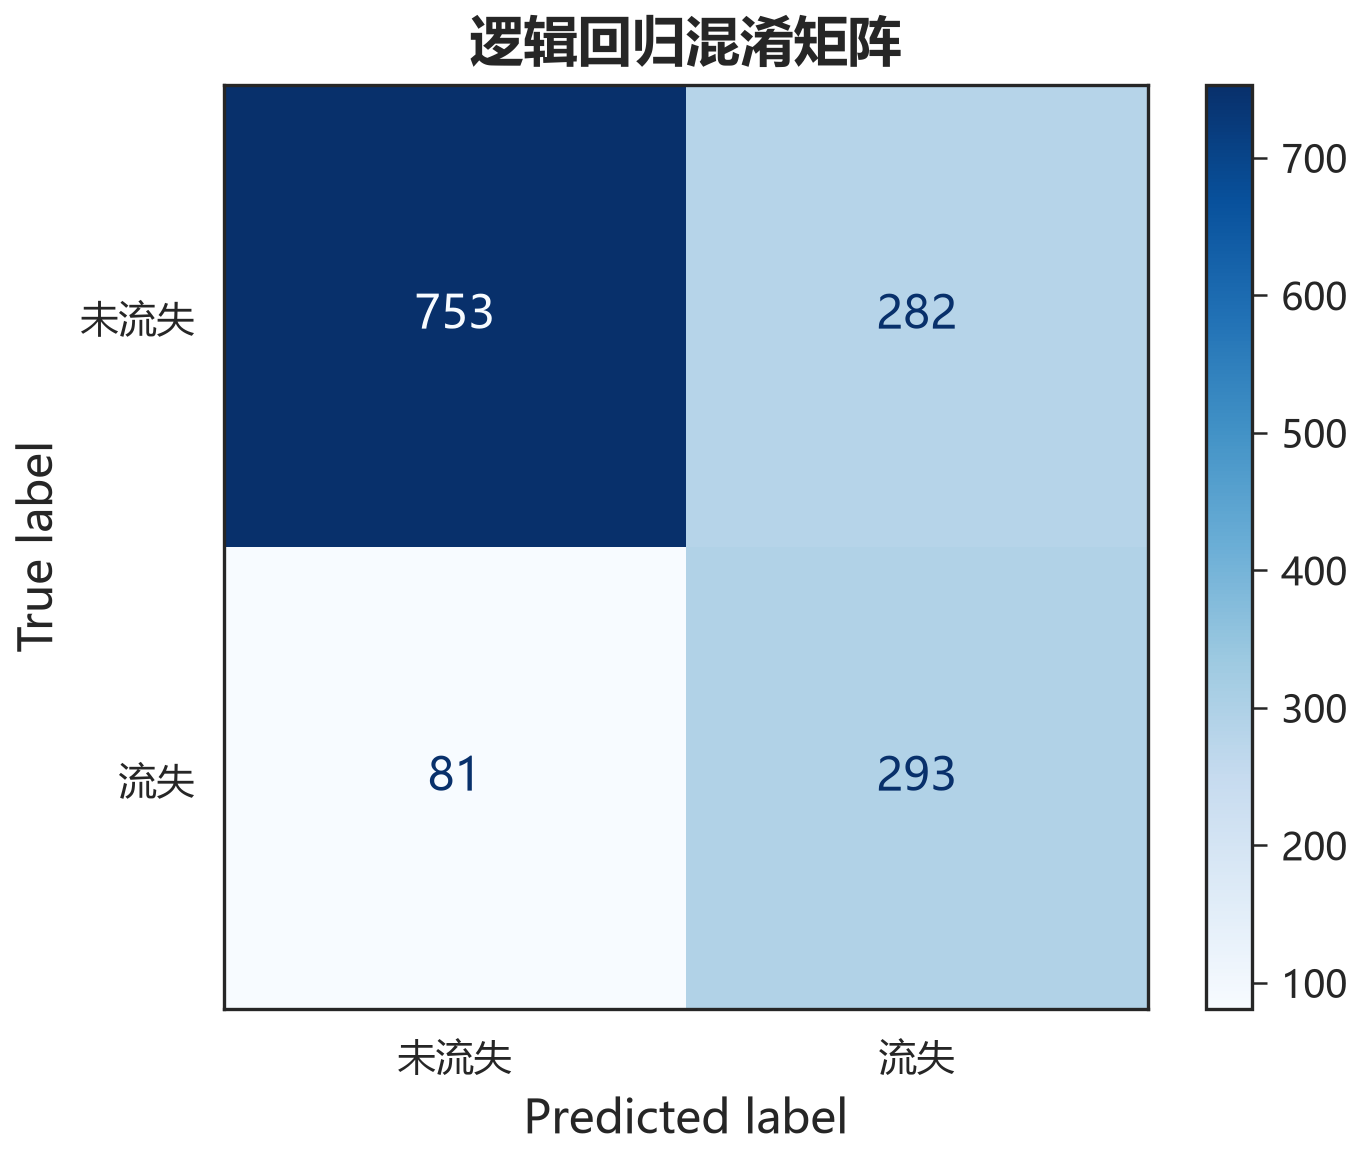
\includegraphics[width=0.5\textwidth]{figures/confusion_matrix.png}
    \caption{逻辑回归混淆矩阵}
    \label{fig:confusion_matrix}
\end{figure}

混淆矩阵的四格分别对应：真阴性（左上，正确预测未流失）、
假阳性（右上，将未流失误判为流失）、假阴性（左下，
将流失误判为未流失）和真阳性（右下，正确预测流失）。
从图中可以看出，模型对未流失客户的分类准确度较高
（左上角数值显著大于右上角），同时得益于
\texttt{class\_weight='balanced'} 的设置，模型也成功识别了
大部分流失客户（右下角），这与表 \ref{tab:lr_metrics} 中
0.78 的召回率相互印证。

\begin{figure}[H]
    \centering
    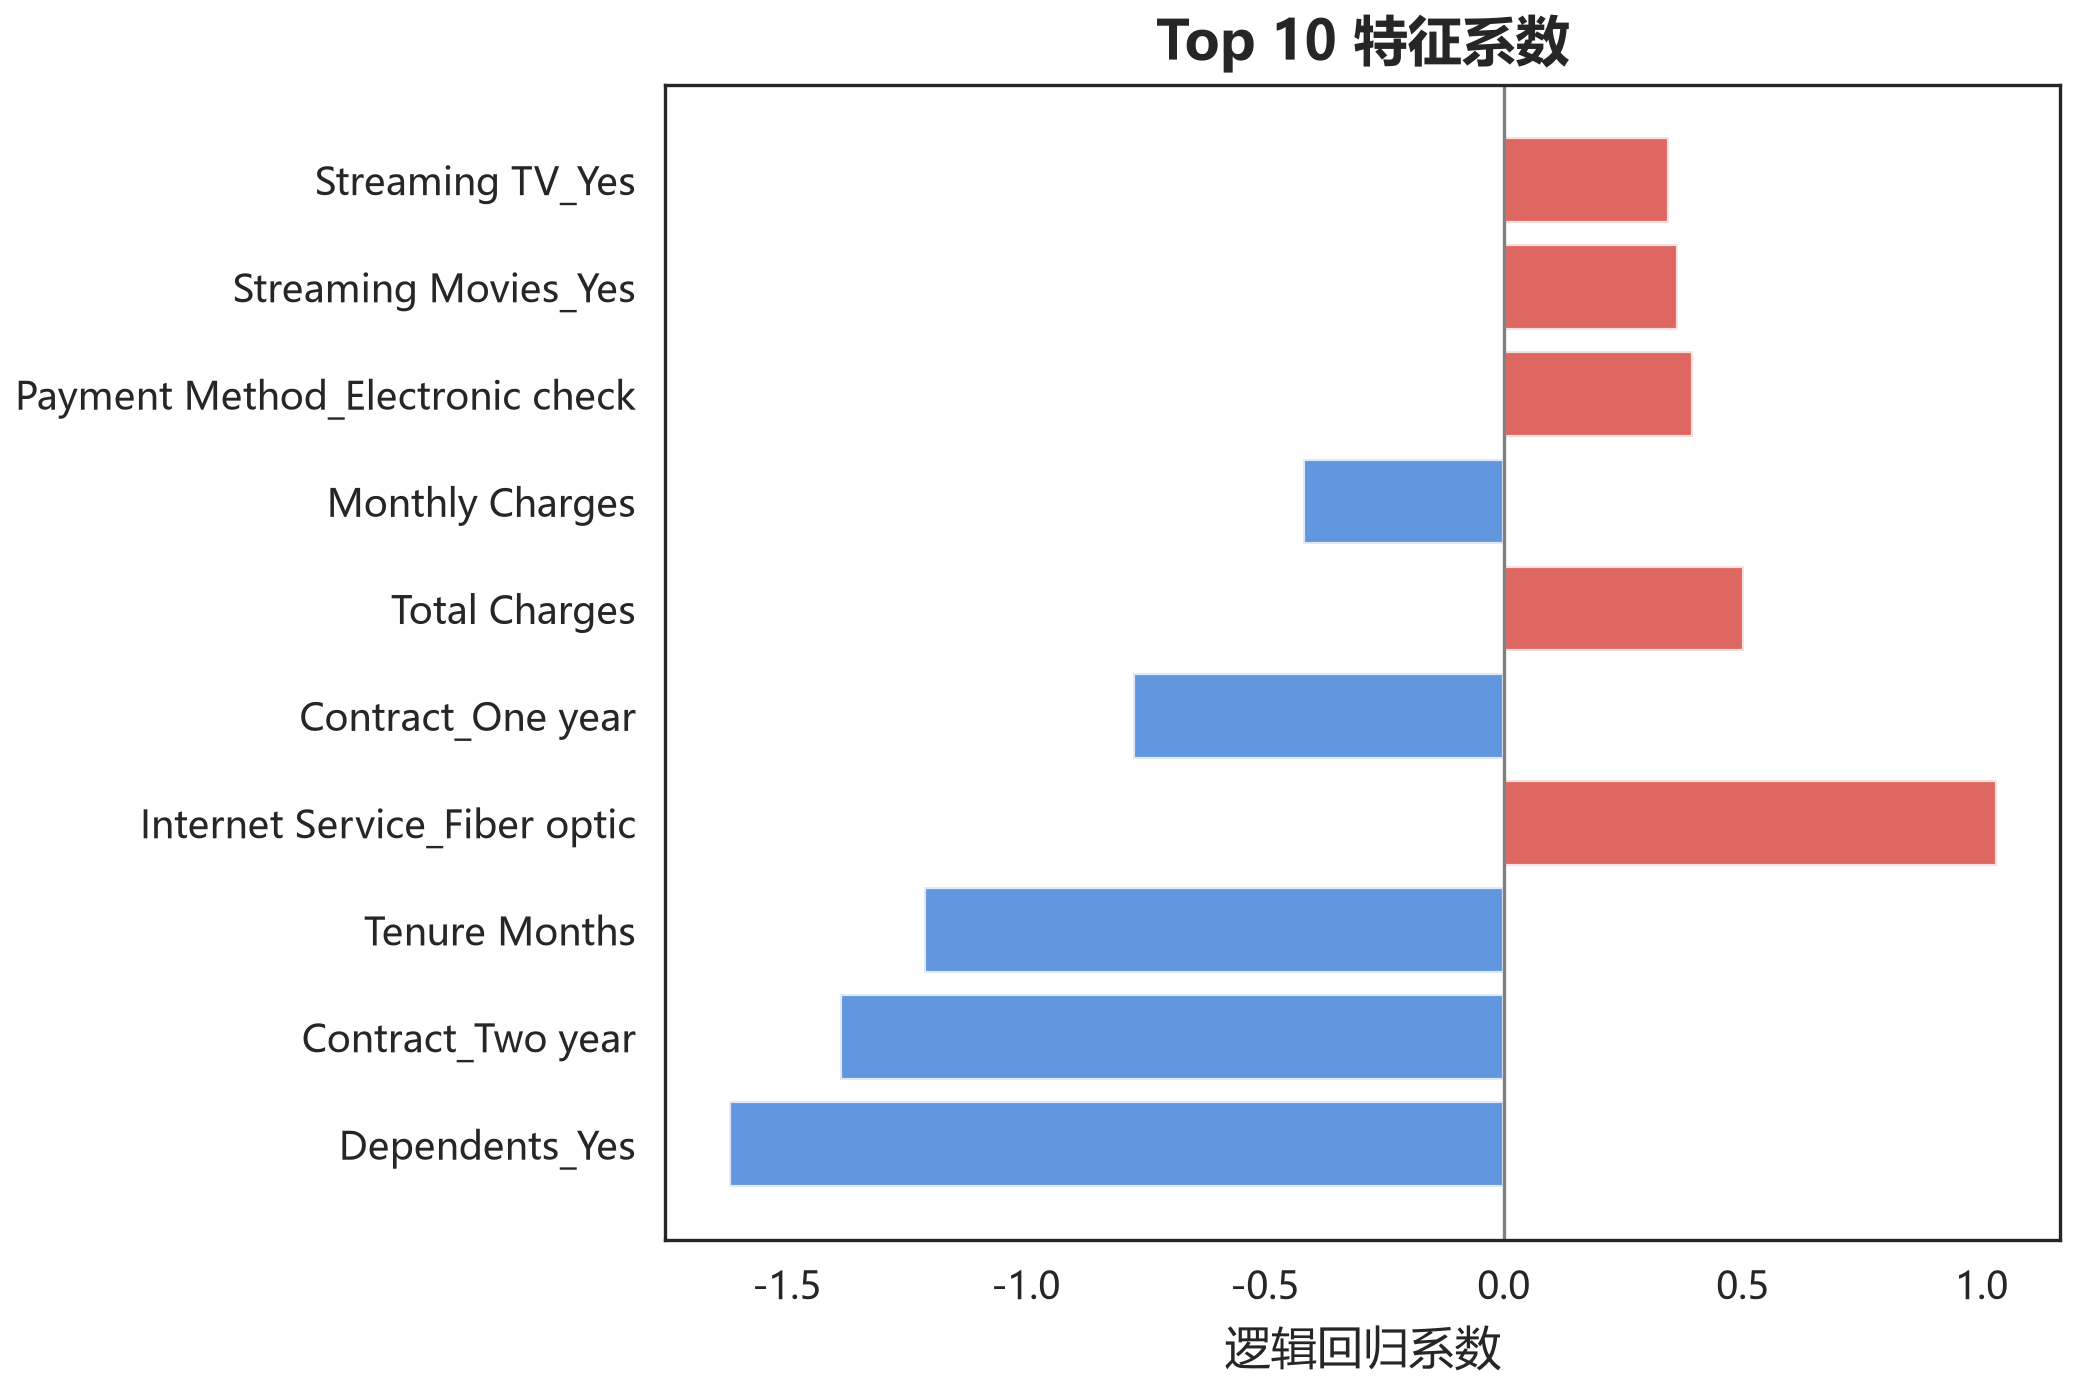
\includegraphics[width=0.65\textwidth]{figures/feature_importance.png}
    \caption{逻辑回归特征系数（Top 10）}
    \label{fig:feature_importance}
\end{figure}

图 \ref{fig:feature_importance} 展示了绝对值最大的前 10 个
逻辑回归系数。蓝色表示负系数——该特征取值增大将降低流失概率，
橙色表示正系数——该特征取值增大将增加流失风险。在网时长的
负系数绝对值最大（约为 $-1.21$），与 EDA 阶段"在网越久越不易
流失"的结论一致；而光纤服务与电子支票支付等特征呈现正系数，
表明这些服务类型本身即关联着较高的流失倾向。需要注意的是，
上述系数受特征间共线性的影响（如在网时长与总消费），
因此仅作为初步参考，更精确的重要性评估将在本节后续通过
SHAP 方法完成。

模型的 AUC 达到 0.849，整体排序能力良好。召回率达到 0.78，
说明模型能够有效识别 78\% 的实际流失客户，具有实用的预警价值。
精确率为 0.51，意味着模型预测为"流失"的客户中约有一半实际
并未流失。从挽留业务的视角来看，误判的代价（向未流失客户
发放挽留优惠）远低于漏判的代价（未能识别出即将流失的客户
而任其离网）。因此，在建模目标上本文优先保证召回率——宁可接受
部分误判带来的额外优惠成本，也要尽可能多地识别出潜在的流失客户，
避免客户离网后更高的替代成本。

\subsection{随机森林与 XGBoost 对比}

随机森林由 Breiman 于 2001 年提出 \cite{breiman2001random}，
其训练过程引入双重随机性——在 Bootstrap 采样的训练子集上，
每棵决策树的分裂仅从随机选取的 $\sqrt{p}$ 个特征中选择最优
分裂点——从而在单棵树容易过拟合的同时，通过集成多棵树的
投票结果获得稳定的整体预测能力。
XGBoost \cite{chen2016xgboost} 是梯度提升树算法的高效实现，
与随机森林并行训练不同，它采用逐轮迭代的方式，使每一棵新树
都去拟合前一棵树的残差，从而逐步降低整体偏差。

仅凭逻辑回归一个模型的评估结果，尚不足以充分判断线性假设
是否已足够刻画该数据集上的流失规律。如果特征之间存在显著的
非线性交互效应，能够捕捉非线性关系的随机森林或 XGBoost
在 AUC 上将明显高于逻辑回归。反之，若三者的 AUC 相近，
则说明线性假设在该问题上是合理的。

\begin{table}[H]
    \centering
    \caption{三模型性能对比}
    \label{tab:model_compare}
    \begin{tabular}{lccc}
        \toprule
        模型 & Accuracy & AUC & F1-score \\
        \midrule
        逻辑回归 & 0.742 & \textbf{0.849} & 0.617 \\
        随机森林 & 0.784 & 0.840 & 0.625 \\
        XGBoost  & 0.750 & 0.847 & 0.622 \\
        \bottomrule
    \end{tabular}
\end{table}

对比结果表明，三者的 AUC 差异不超过 0.01，F1-score 同样高度接近
（均在 0.62 左右）。逻辑回归（AUC=0.849）甚至略高于随机森林
（AUC=0.840）和 XGBoost（AUC=0.847），这说明在该数据集上各特征
与流失概率之间以线性关系为主导，复杂的非线性交互效应并不显著。
因此，逻辑回归不仅具有最强的可解释性，在预测精度上也未因线性
假设的简化而损失性能，适合作为本文的最终预测模型。

\begin{figure}[H]
    \centering
    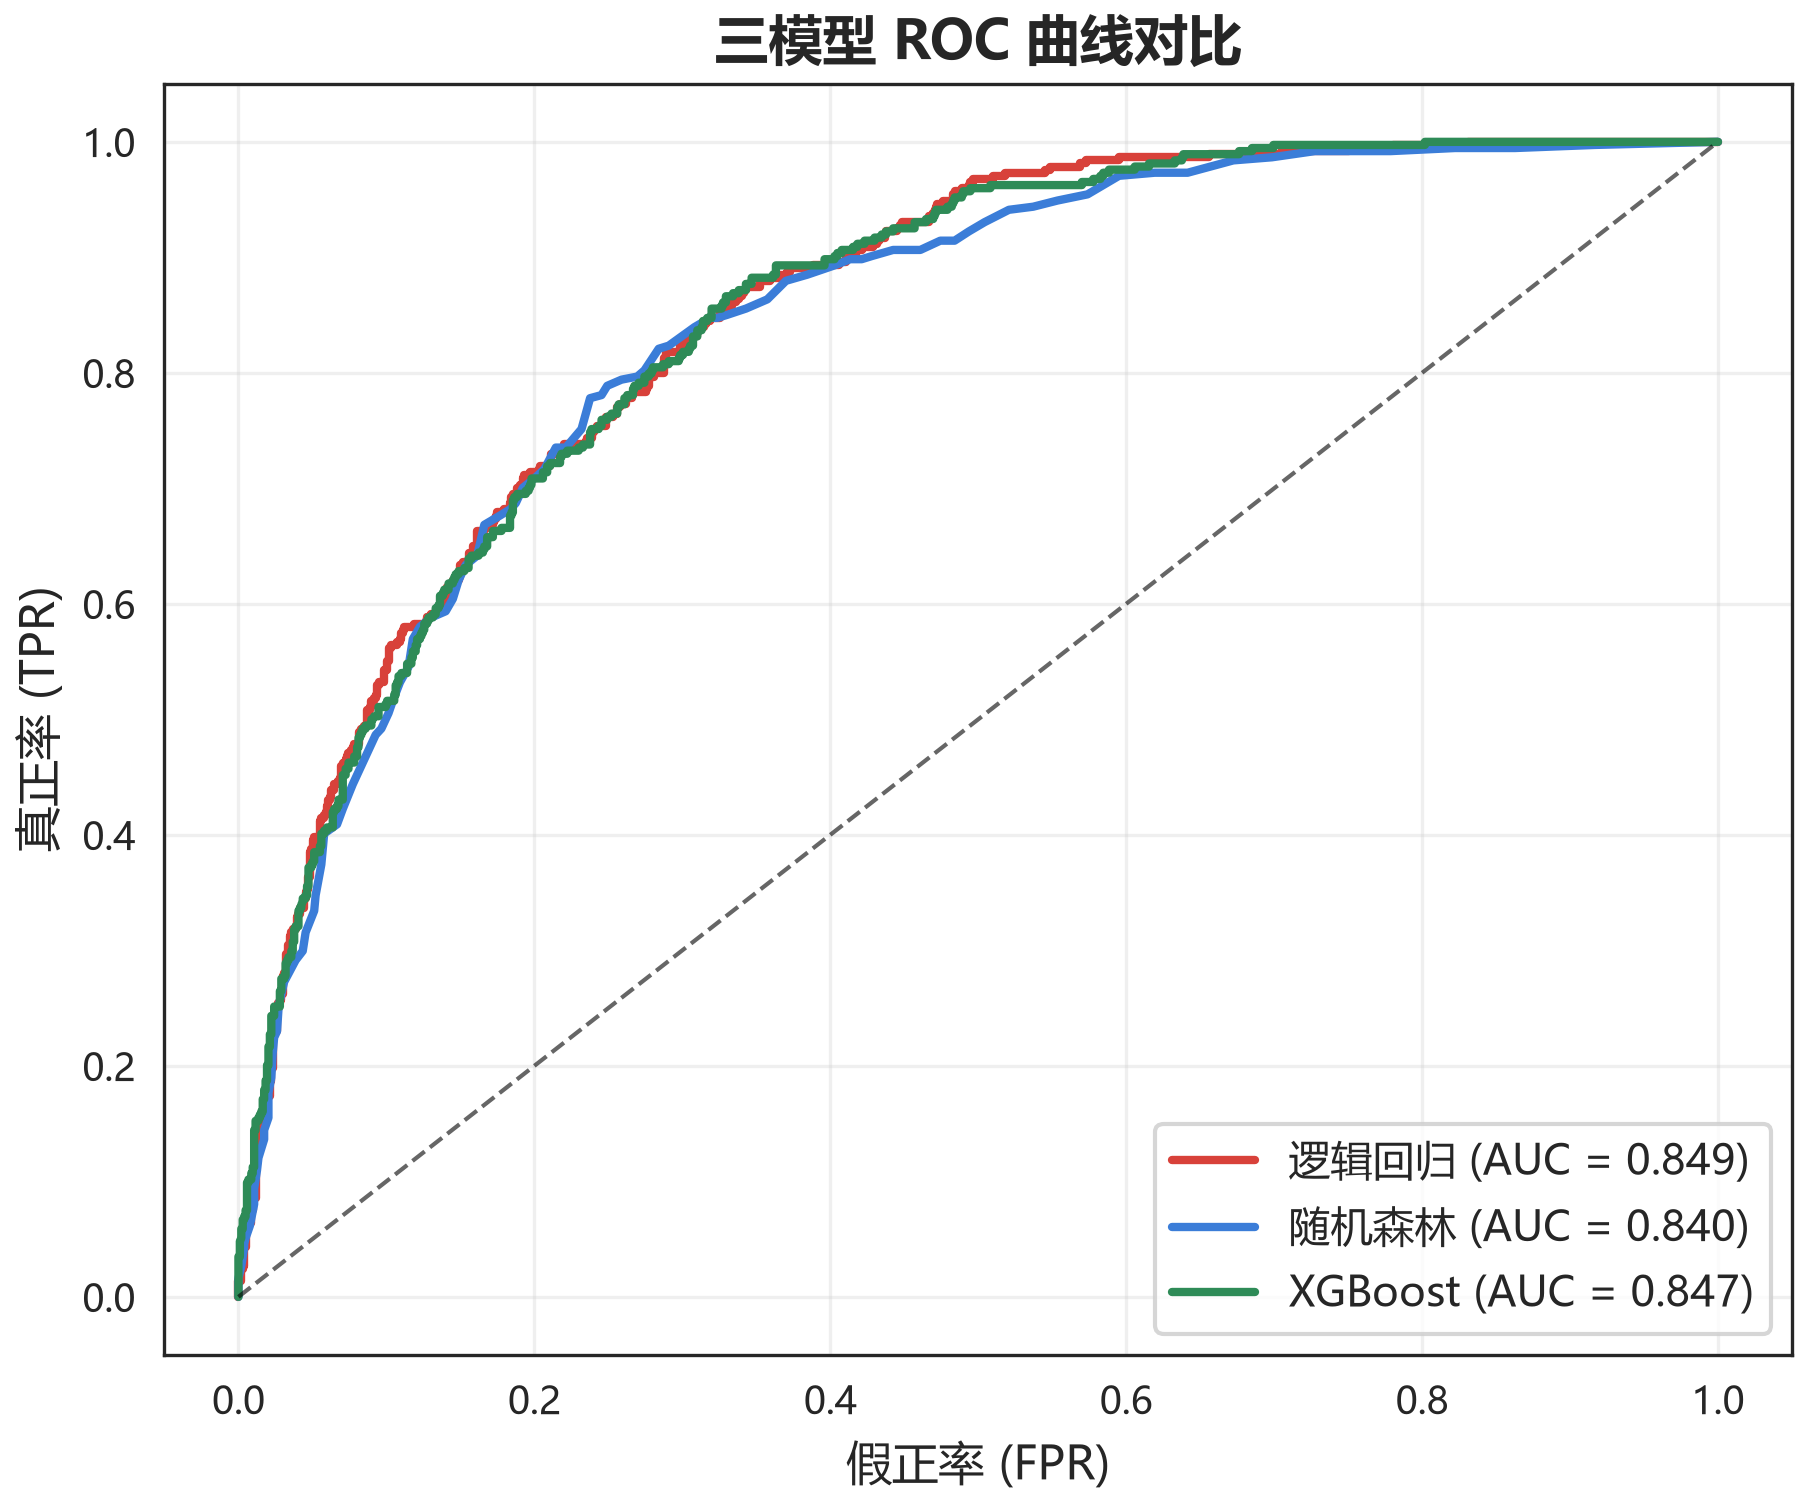
\includegraphics[width=0.7\textwidth]{figures/roc_compare.png}
    \caption{三模型 ROC 曲线对比}
    \label{fig:roc_compare}
\end{figure}

如图 \ref{fig:roc_compare} 所示，三条 ROC 曲线均显著高于随机
猜测线（对角线），且曲线间几乎完全重叠——逻辑回归（AUC=0.849）
与 XGBoost（AUC=0.847）仅差 0.002。F1-score 方面，三者也高度
接近（0.617 -- 0.625）。ROC 曲线和 F1 的双重证据一致表明：
在该数据集上，线性假设已足够刻画流失规律，引入非线性模型并未
带来实质性的预测增益。

\subsection{关键流失因子识别}

在确定逻辑回归为最终模型后，接下来需要量化各特征对流失风险的
具体贡献，即识别前五位关键流失驱动因素。

逻辑回归的系数 $\beta_j$ 虽然能够反映各特征的影响方向，但直接
使用系数进行跨特征的重要性比较存在两个问题：一是不同特征量纲
不同，系数绝对值大小受标准化方式影响；二是在网时长与总消费之间
的相关系数高达 0.83，高度的共线性会导致两特征的系数出现不稳定
的符号或大小，因此不能仅凭系数值判定哪个特征更"重要"。

为此，本文引入 SHAP（SHapley Additive exPlanations）
\cite{lundberg2017unified} 对逻辑回归的输出进行归因分析。
SHAP 将合作博弈中的 Shapley 公平分配原则迁移到模型解释场景：
把任意样本的预测值拆分为各特征的边际效应之和，
从而在消除量纲差异与共线性干扰的条件下，
完成特征间无偏的重要性排序。本文采用与线性模型匹配的
LinearExplainer 进行全局与局部两层分析。

\begin{figure}[H]
    \centering
    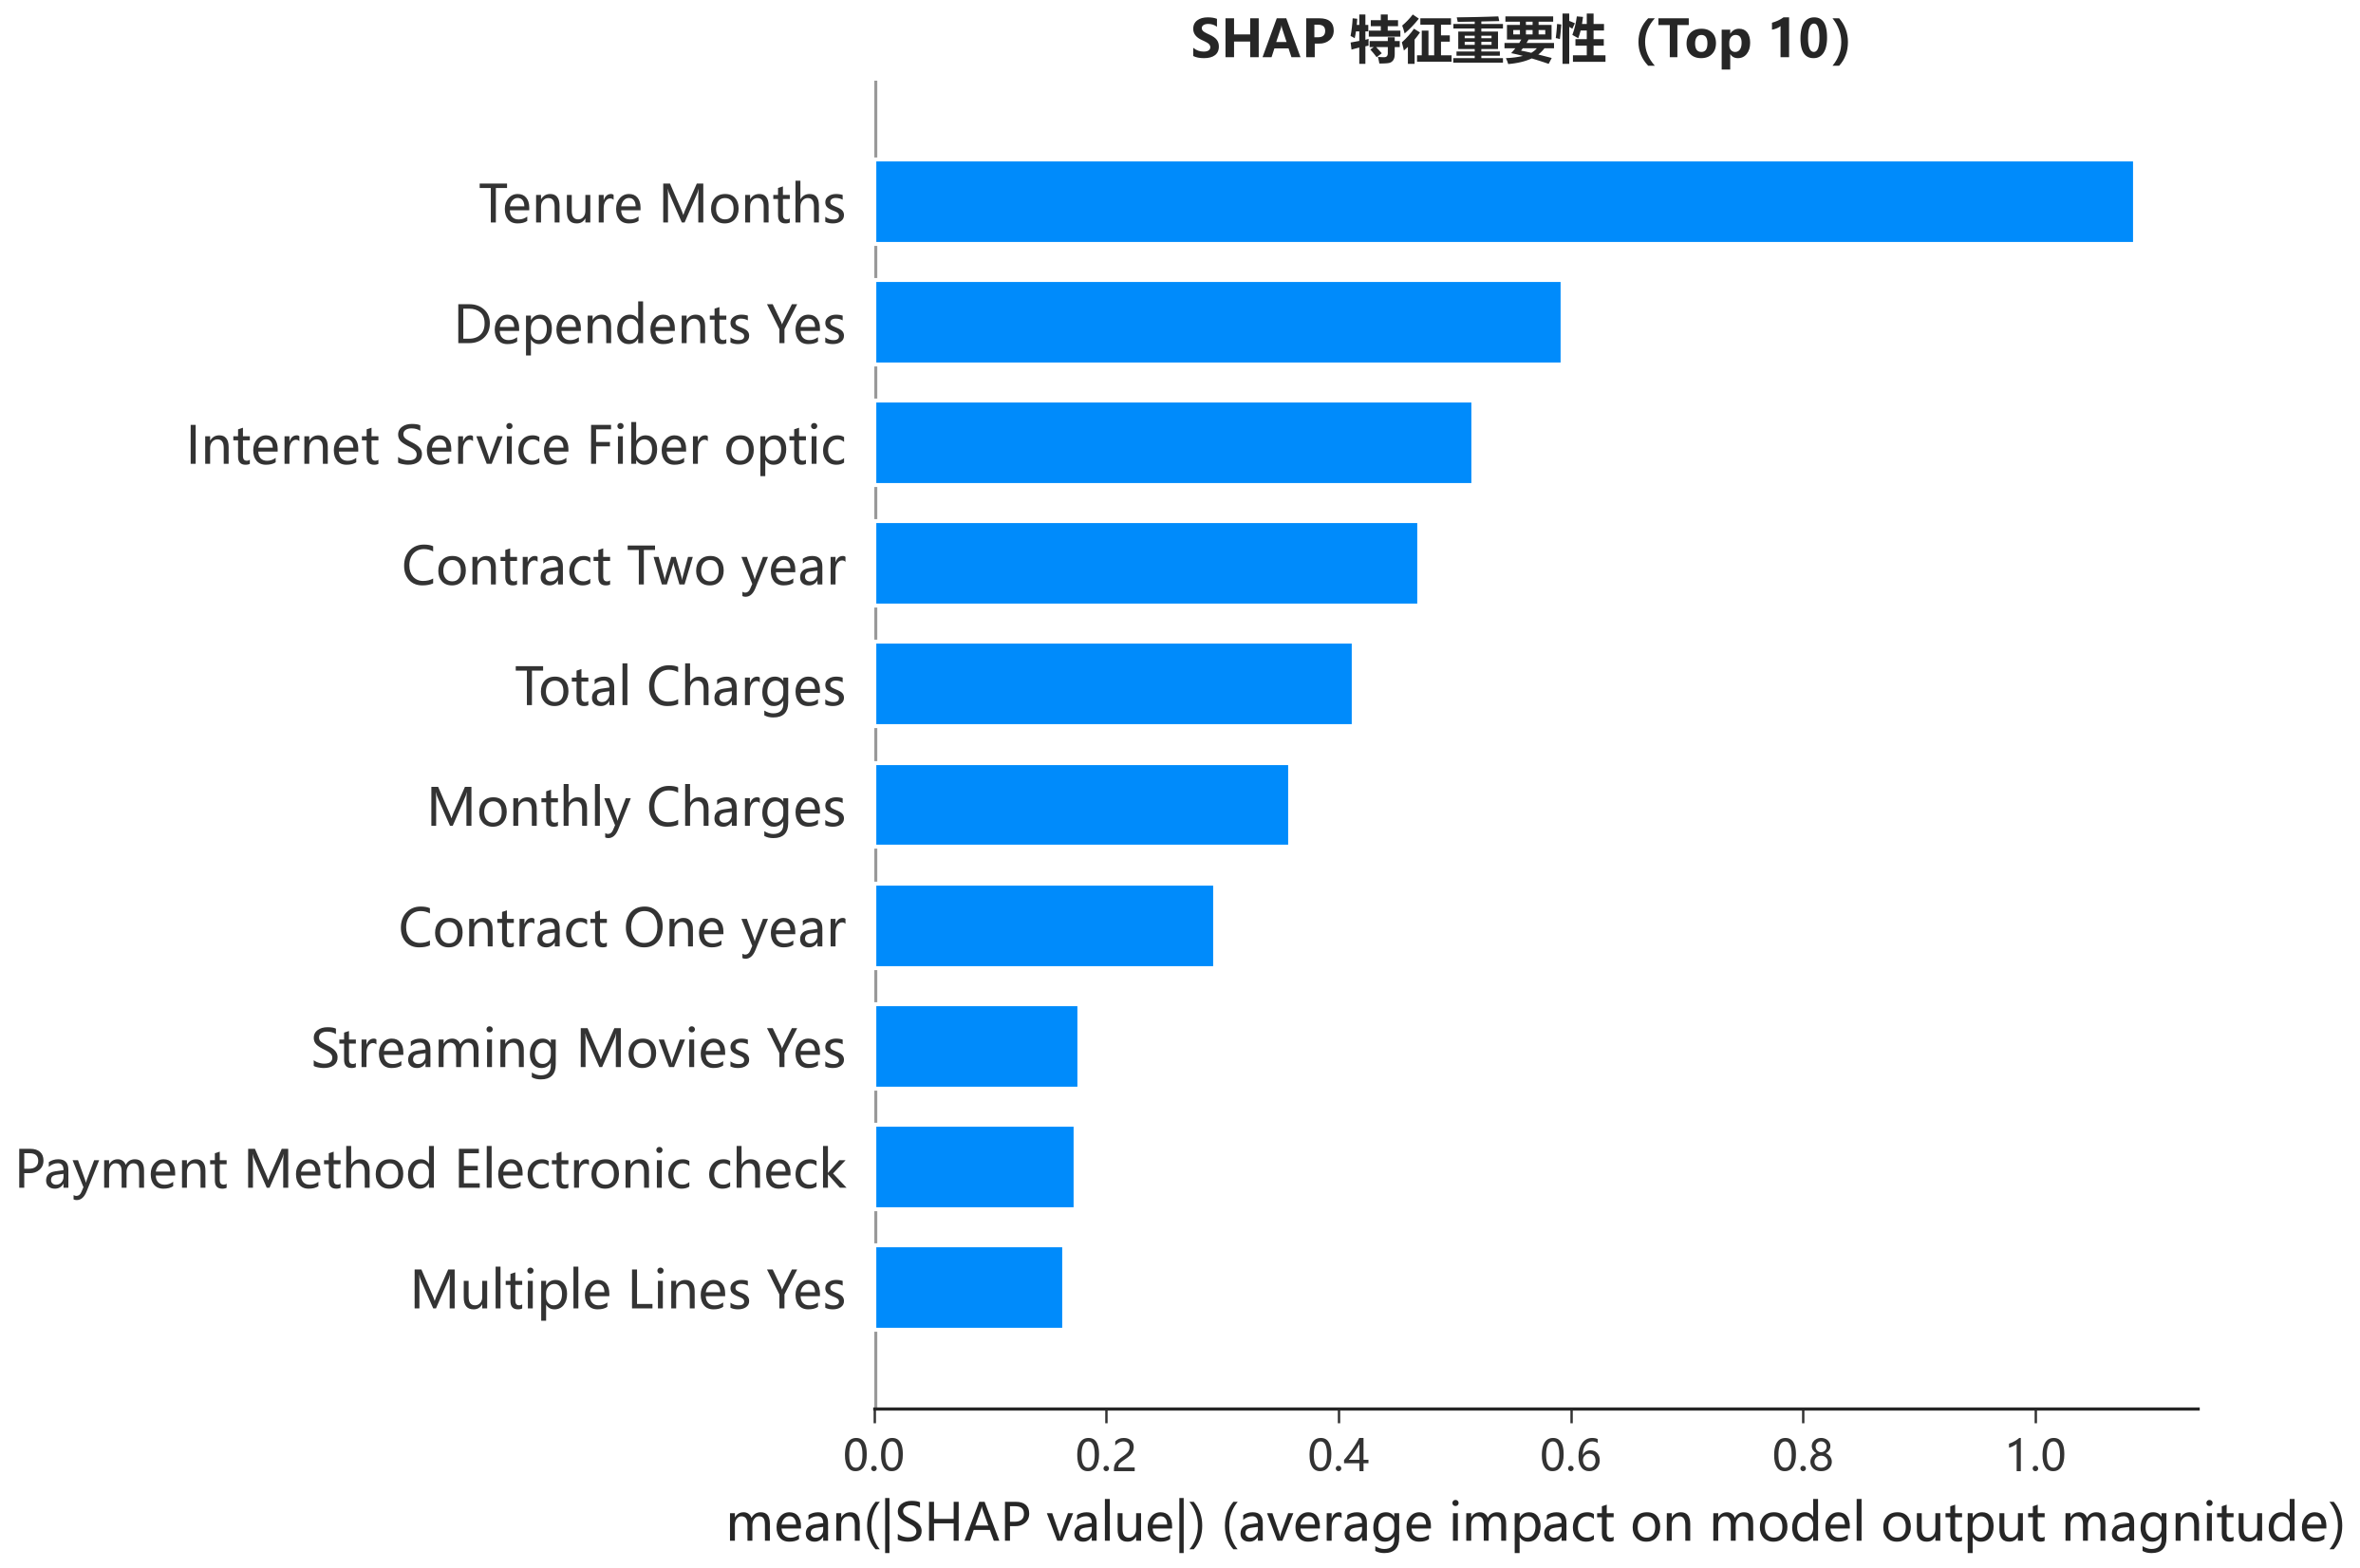
\includegraphics[width=0.7\textwidth]{figures/shap_bar.png}
    \caption{SHAP 特征重要性排序（Top 10）}
    \label{fig:shap_bar}
\end{figure}

如图 \ref{fig:shap_bar} 所示，在网时长的平均 SHAP 绝对值
（约 1.09）远高于其他特征，呈现"一家独大"的格局。此外，
前五位特征中包含两个合同相关变量（两年合同、光纤服务）和
一个家庭/人口变量（家属），与问题一中 EDA 的分类特征分析
和相关性分析在定性结论上完整一致。SHAP 排序在保留方向性
信息的同时，利用 Shapley 值的公平分配机制克服了多重共线性
的干扰（在网时长与总消费的 $r=0.83$），因而排序比原始逻辑
回归系数更可靠。

\begin{figure}[H]
    \centering
    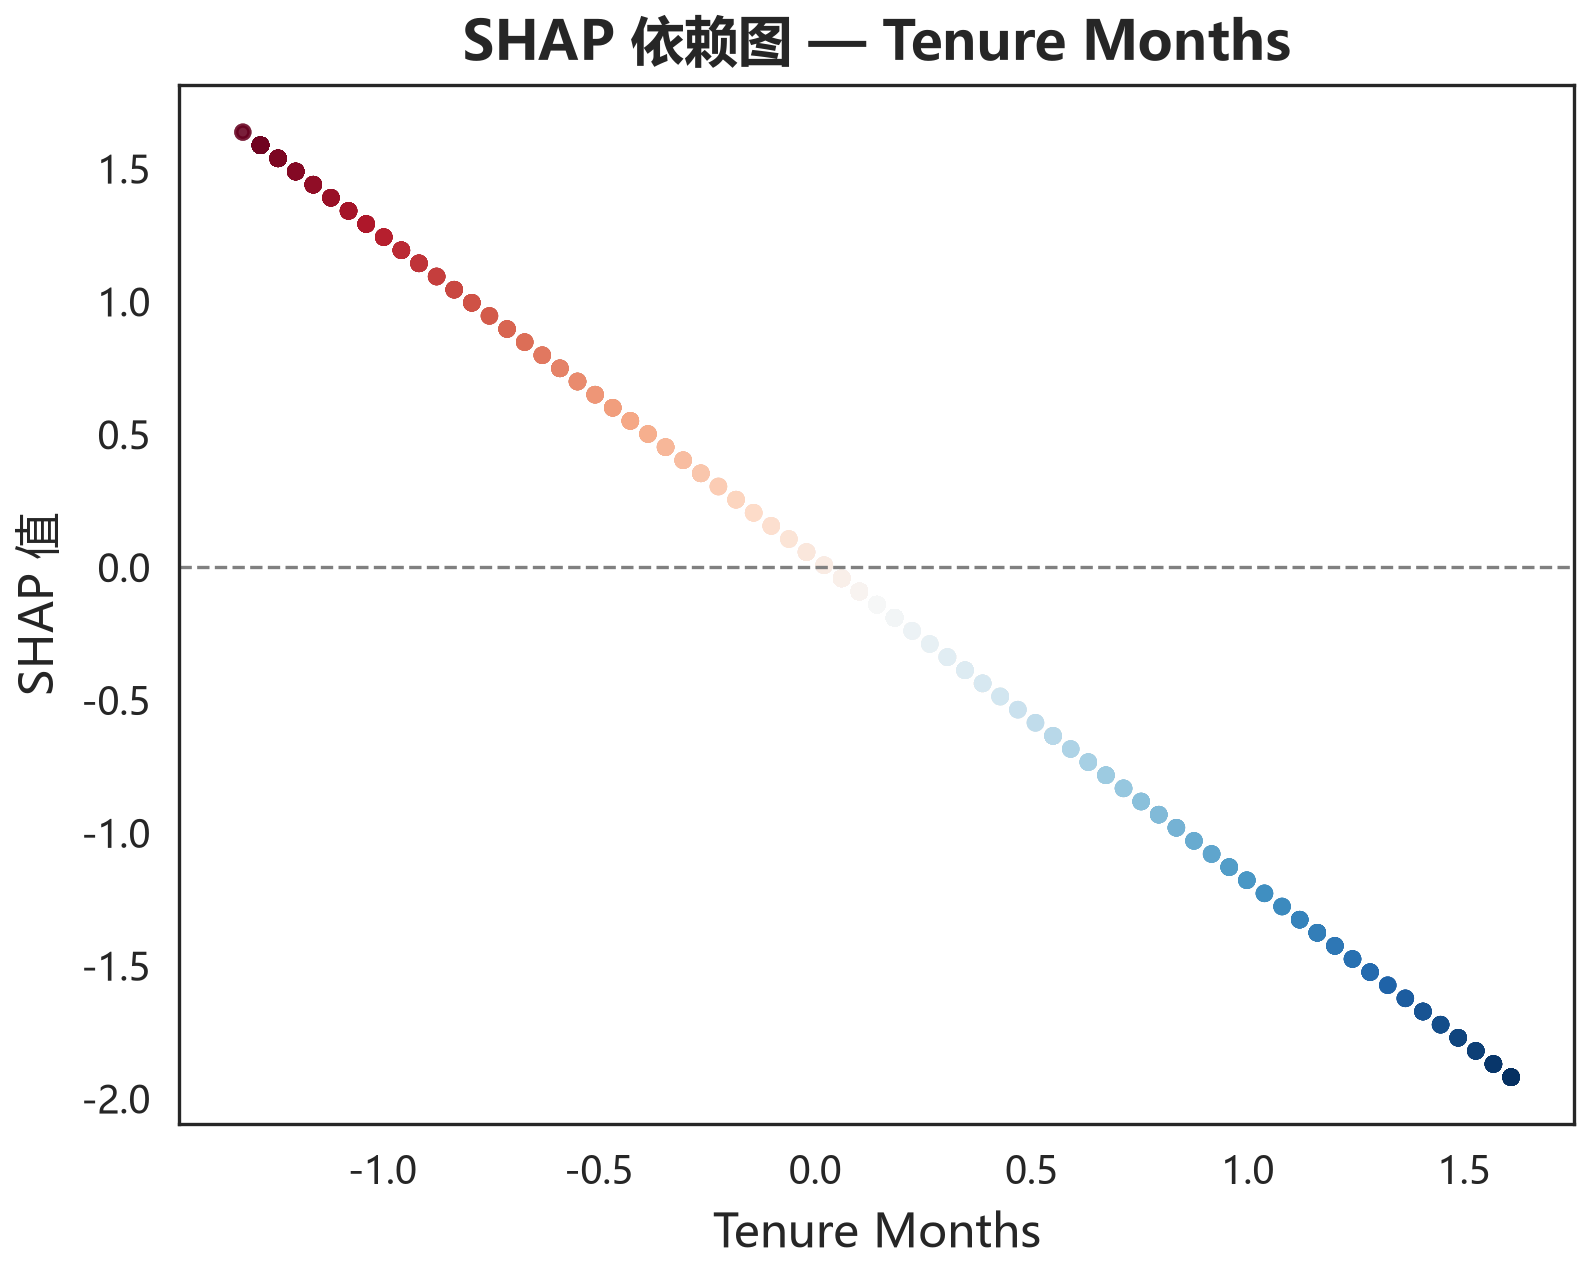
\includegraphics[width=0.65\textwidth]{figures/shap_Tenure_Months.png}
    \caption{在网时长的 SHAP 依赖图}
    \label{fig:shap_tenure}
\end{figure}

图 \ref{fig:shap_tenure} 展示了在网时长的 SHAP 依赖图：
横轴为在网月数，纵轴为该特征对每个样本流失概率的贡献值。
SHAP 值在前 10 个月内高度集中于正值区间（$> 0$），表明在网
时间短的客户被模型系统性判定为高流失风险；随着在网月数突破
24 个月，SHAP 值全面转负且趋于平稳，流失风险的边际递减效应
趋于饱和。这一模式与问题一的直方图发现——"流失客户高度集中
于 0--10 个月"——高度吻合，进一步证实在网时长的首年是客户
关系最脆弱的窗口期。

\begin{figure}[H]
    \centering
    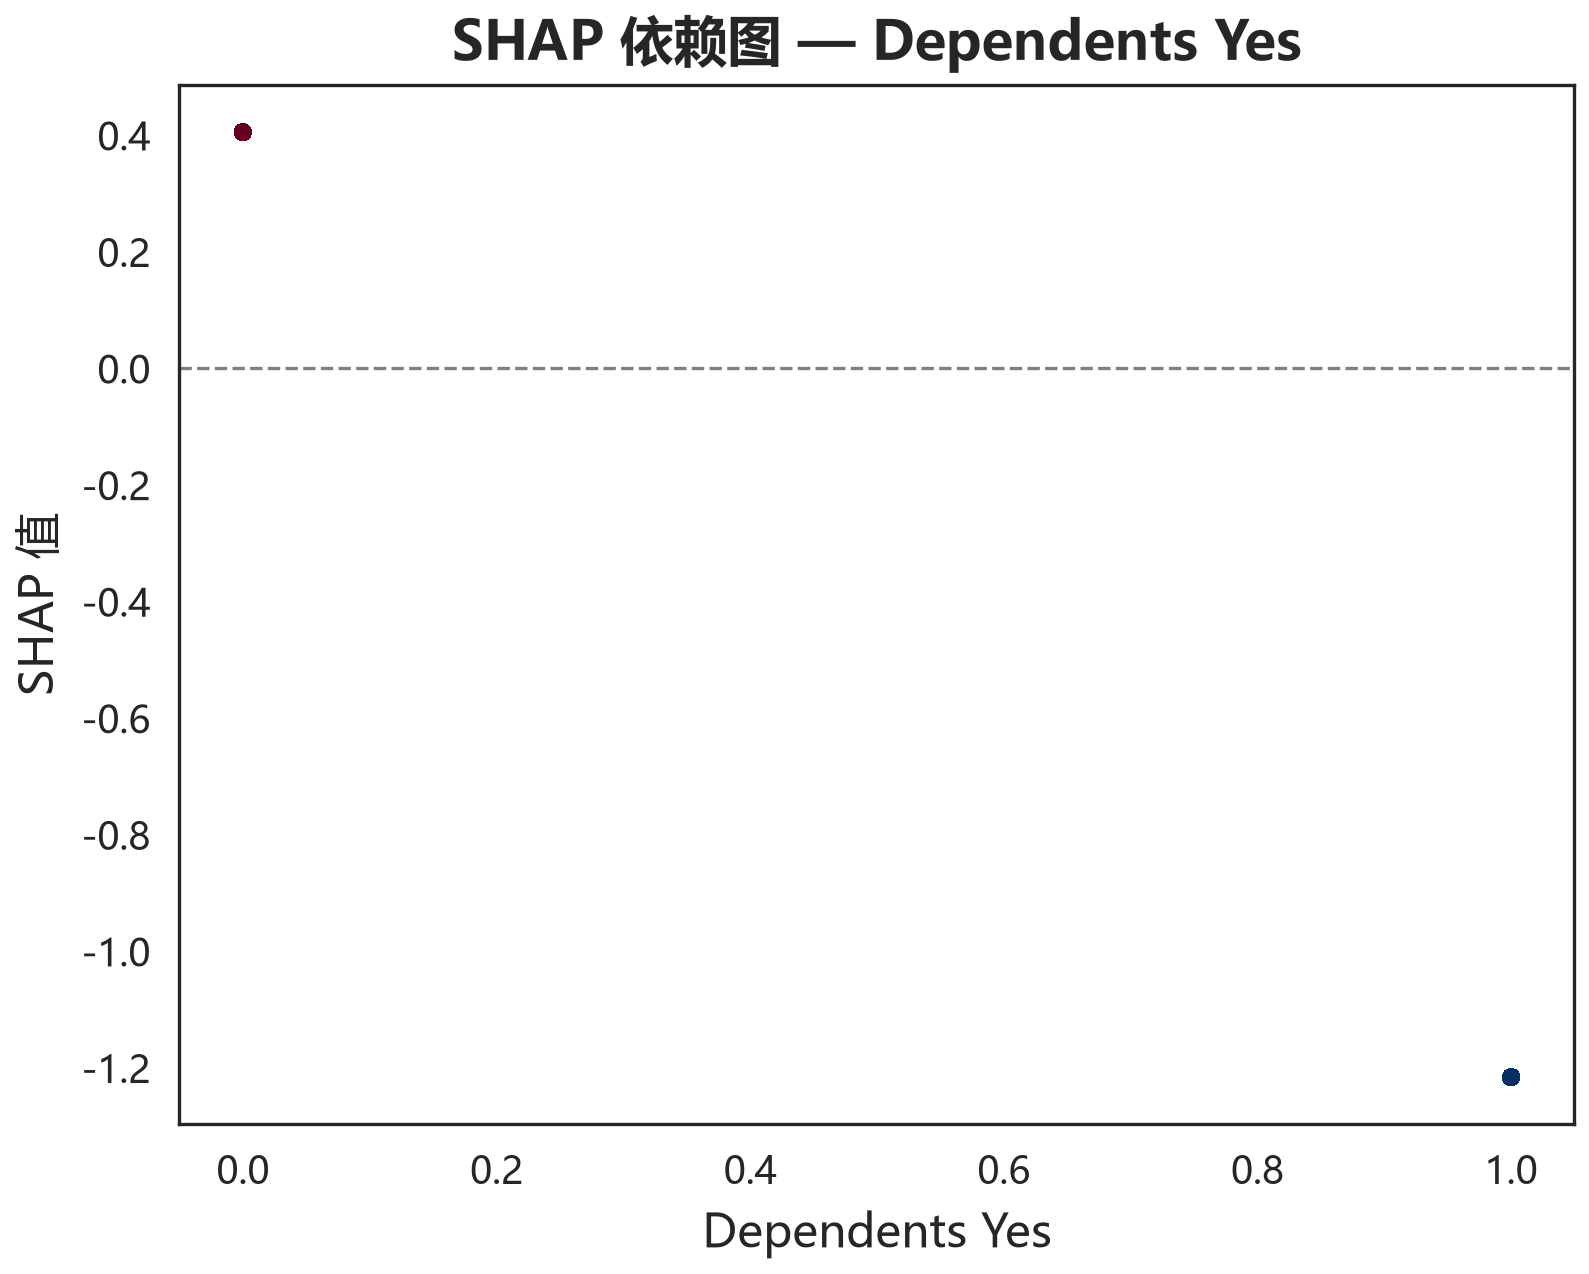
\includegraphics[width=0.65\textwidth]{figures/shap_Dependents_Yes.png}
    \caption{是否有家属的 SHAP 依赖图}
    \label{fig:shap_dependents}
\end{figure}

家有家属（Dependents = Yes）的客户 SHAP 值系统性为负，
分布宽度较窄（约 $-0.8$ 至 $-0.3$），效应方向一致且稳定。
说明家庭责任赋予了一种额外的"锁定效应"——有子女或赡养义务
的客户更换运营商的决策成本更高，与问题一中"有家属客户流失率
更低"的柱状图结论相互印证。这一发现为挽留策略中"家庭套餐
优先推广"提供了直接的量化依据。

\subsubsection*{Top 5 关键流失因子}

综合 SHAP 分析结果，各特征的平均 SHAP 绝对值由大到小排序，
前五位关键流失因子及其业务解读如表 \ref{tab:top5} 所示。

\begin{table}[H]
    \centering
    \caption{Top 5 关键流失因子}
    \label{tab:top5}
    \small
    \begin{tabular}{clp{7cm}}
        \toprule
        排名 & 特征 & 业务解读 \\
        \midrule
        1 & 在网时长 &
        SHAP=1.09，负向。在网越短流失概率越高，与 EDA 中
        相关系数 $-0.352$ 及"0-10 个月高度集中"的直方图分布
        一致。运营商应重点关注入网首年的客户运营和关怀。
        \\
        2 & 是否有家属（是） &
        SHAP=0.59，负向。有家庭成员绑定的客户离网意愿更低，
        与分类特征分析中"有家属客户流失率更低"的结论一致。
        家庭套餐与捆绑服务是降低流失的有效手段。
        \\
        3 & 互联网服务（光纤） &
        SHAP=0.52，正向。光纤客户流失风险显著高于 DSL 客户，
        与分类特征分析中光纤流失率约 30\%、DSL 约 15\% 的
        对比一致。建议检查光纤服务的定价合理性和服务质量。
        \\
        4 & 合同类型（两年） &
        SHAP=0.47，负向。两年合同客户流失率不到 3\%，
        与三种合同类型明显的流失率梯度（月付 > 40\%、一年
        ~10\%、两年 ~3\%）一致。引导客户从月付转向长约
        是最有效的挽留手段之一。
        \\
        5 & 总消费金额 &
        SHAP=0.41，方向混合。总消费体现客户累积投入，
        高消费客户粘性相对较高，但需注意其与在网时长的
        共线性（$r=0.83$），部分贡献可能来源于在网时长的
        间接效果。
        \\
        \bottomrule
    \end{tabular}
\end{table}

上述 SHAP 分析得出的 Top 5 排序与问题一中各阶段的结论形成了
多层次的交叉验证：在网时长的最强区分能力同时被相关系数
（$-0.352$）、分组直方图和 SHAP 重要性三种不同方法共同确认；
合同类型和家属情况的显著影响在分类特征对比图和 SHAP 排序中
得到一致反映；光纤服务的高流失风险在流失率柱状图和 SHAP
重要性中均得到体现。这种"探索性分析 → 建模量化"的两阶段
验证策略表明，模型学到的规律并非偶然，而是数据内在结构在
两种不同分析框架下的稳定呈现。
